\documentclass[letterpaper, 10 pt, conference]{ieeeconf}
\IEEEoverridecommandlockouts
\overrideIEEEmargins

%In case you encounter the following error:
%Error 1010 The PDF file may be corrupt (unable to open PDF file) OR
%Error 1000 An error occurred while parsing a contents stream. Unable to analyze the PDF file.
%This is a known problem with pdfLaTeX conversion filter. The file cannot be opened with acrobat reader
%Please use one of the alternatives below to circumvent this error by uncommenting one or the other
%\pdfobjcompresslevel=0
%\pdfminorversion=4

% The following packages can be found on http:\\www.ctan.org
\usepackage{graphics} % for pdf, bitmapped graphics files
\usepackage{epsfig} % for postscript graphics files
\usepackage{mathptmx} % assumes new font selection scheme installed
\usepackage{times} % assumes new font selection scheme installed
\usepackage{amsmath} % assumes amsmath package installed
\usepackage{amssymb}  % assumes amsmath package installed
\usepackage{multirow}
\usepackage{booktabs}
\usepackage{float}
\usepackage{threeparttable}

\usepackage{cite}
%\usepackage[square, comma, sort&compress, numbers]{natbib}

\usepackage{color, soul}
\sethlcolor{blue}
\newcommand{\hlr}[1]{{\color{red}{#1}}}

%\usepackage{spconf,amsmath,graphicx}
%\usepackage{amssymb}

\title{\LARGE \bf
Coarse-to-fine Semantic Localization with HD Map for Autonomous Driving In the Structured Scene
}


\author{Chengcheng Guo, Minjie Lin, Heyang Guo, Pengpeng Liang and Erkang Cheng% <-this % stops a space
%\thanks{*This work was not supported by any organization}% <-this % stops a space
\thanks{Chengcheng Guo, Minjie Lin, Heyang Guo and Erkang Cheng are with the NullMax, Shanghai, 201210, China. Pengpeng Liang is with Zhengzhou University.
        {\tt\small guochengcheng, linminjie, guoheyang, chengerkang@nullmax.ai; liangpcs@gmail.com}}%
}


\begin{document}


\maketitle
\thispagestyle{empty}
\pagestyle{empty}


%%%%%%%%%%%%%%%%%%%%%%%%%%%%%%%%%%%%%%%%%%%%%%%%%%%%%%%%%%%%%%%%%%%%%%%%%%%%%%%%
\begin{abstract}
Robust and accurate localization is an essential component for robotic navigation and autonomous driving. The use of cameras for localization with high definition map (HD Map) provides an affordable localization sensor set. Existing methods suffer from pose estimation failure due to error prone data association or initialization with accurate initial pose requirement. In this paper, we propose a cost-effective vehicle localization system with HD map for autonomous driving that uses cameras as primary sensors. To this end, we formulate vision-based localization as a data association problem that maps visual semantics to landmarks in HD map. Specifically, system initialization is finished in a coarse to fine manner by combining coarse GPS (Global Positioning System) measurement and fine pose searching. In tracking stage, vehicle pose is refined by implicitly aligning the semantic segmentation result between image and landmarks in HD maps with photometric consistency. Finally, vehicle pose is computed by pose graph optimization in a sliding window fashion. We evaluate our method on two datasets and demonstrate that the proposed approach yields promising localization results in different driving scenarios. Additionally, our approach is suitable for both monocular camera and multi-cameras that provides flexibility and improves robustness for the localization system. 

% \hlr{How flexibility is achieved?}


% \hlr{Questions: Is this the first work to mainly use cameras for localization for autonomous driving? If it is, you need to highlight this; otherwise, from the abstract, it is hard to see what problems this paper tries to solve.}

%Vehicle localization (i.e., position and orientation estimation in the world coordinate system) is achieved by camera as main sensor and GNSS used for system initialization.

%We propose a vision localization method which combine semantic segmentation of image and landmarks in vector format hdmap to estimate the vehicle's exact position and orientation in high precision map. The low-cost GNSS data is used for system initialization, then exhaustive pose search is applied to find better vehicle initial pose in a coarse to fine way. 

%In tracking stage, vehicle odometry information is used for pose prediction, then vehicle pose is corrected by aligning semantic elements in map with feature map image based on photometric consistency, which solve the data association (landmark in hd-map, semantic seg) problem dynamic and implicitly. 

%Finally, smooth and robust pose is obtained based on the pose graph optimization in a sliding window. 

%The system is designed not only for monocular camera but also multiple cameras, which improve the robustness and flexibility of system.

%Evaluation on different datasets showed that the method is robust and accurate in different driving scenes, archive the accuracy level of autonomous driving. 
 
 %As far as we know, proposed vision localization system is the most complete, robust and lightweight vision based localization system for autonomous driving. 

\end{abstract}


%%%%%%%%%%%%%%%%%%%%%%%%%%%%%%%%%%%%%%%%%%%%%%%%%%%%%%%%%%%%%%%%%%%%%%%%%%%%%%%%
\section{INTRODUCTION}
%Mapping and localization are basic components of autonomous driving. Accurate and robust localization of the vehicle in HD map can have a positive impact on the decision-making and perception module of autonomous driving. Although the inertial navigation system based on IMU and RTK-GNSS can obtain enough accuracy. However, its high cost make it difficult to applied in large-scale commercial mass production. At the same time, it is difficult to estimate vehicle's pose in places with poor GNSS signal, such as tunnels and skyscraper region\cite{jeong2019complex}.

Vehicle localization (i.e., position and orientation estimation in the world coordinate system) is an important component of the autonomous driving system. For example, accurate and robust localization can provide useful information of decision making and perception module for autonomous driving.
Although the inertial navigation system based on IMU and RTK-GNSS can obtain enough accuracy, it is likely to fail in scenarios with poor GNSS signal, such as tunnels and skyscraper region \cite{jeong2019complex}. Also, it is not cost-effective for massive production. 
 
\begin{figure}[htb]
  \centering{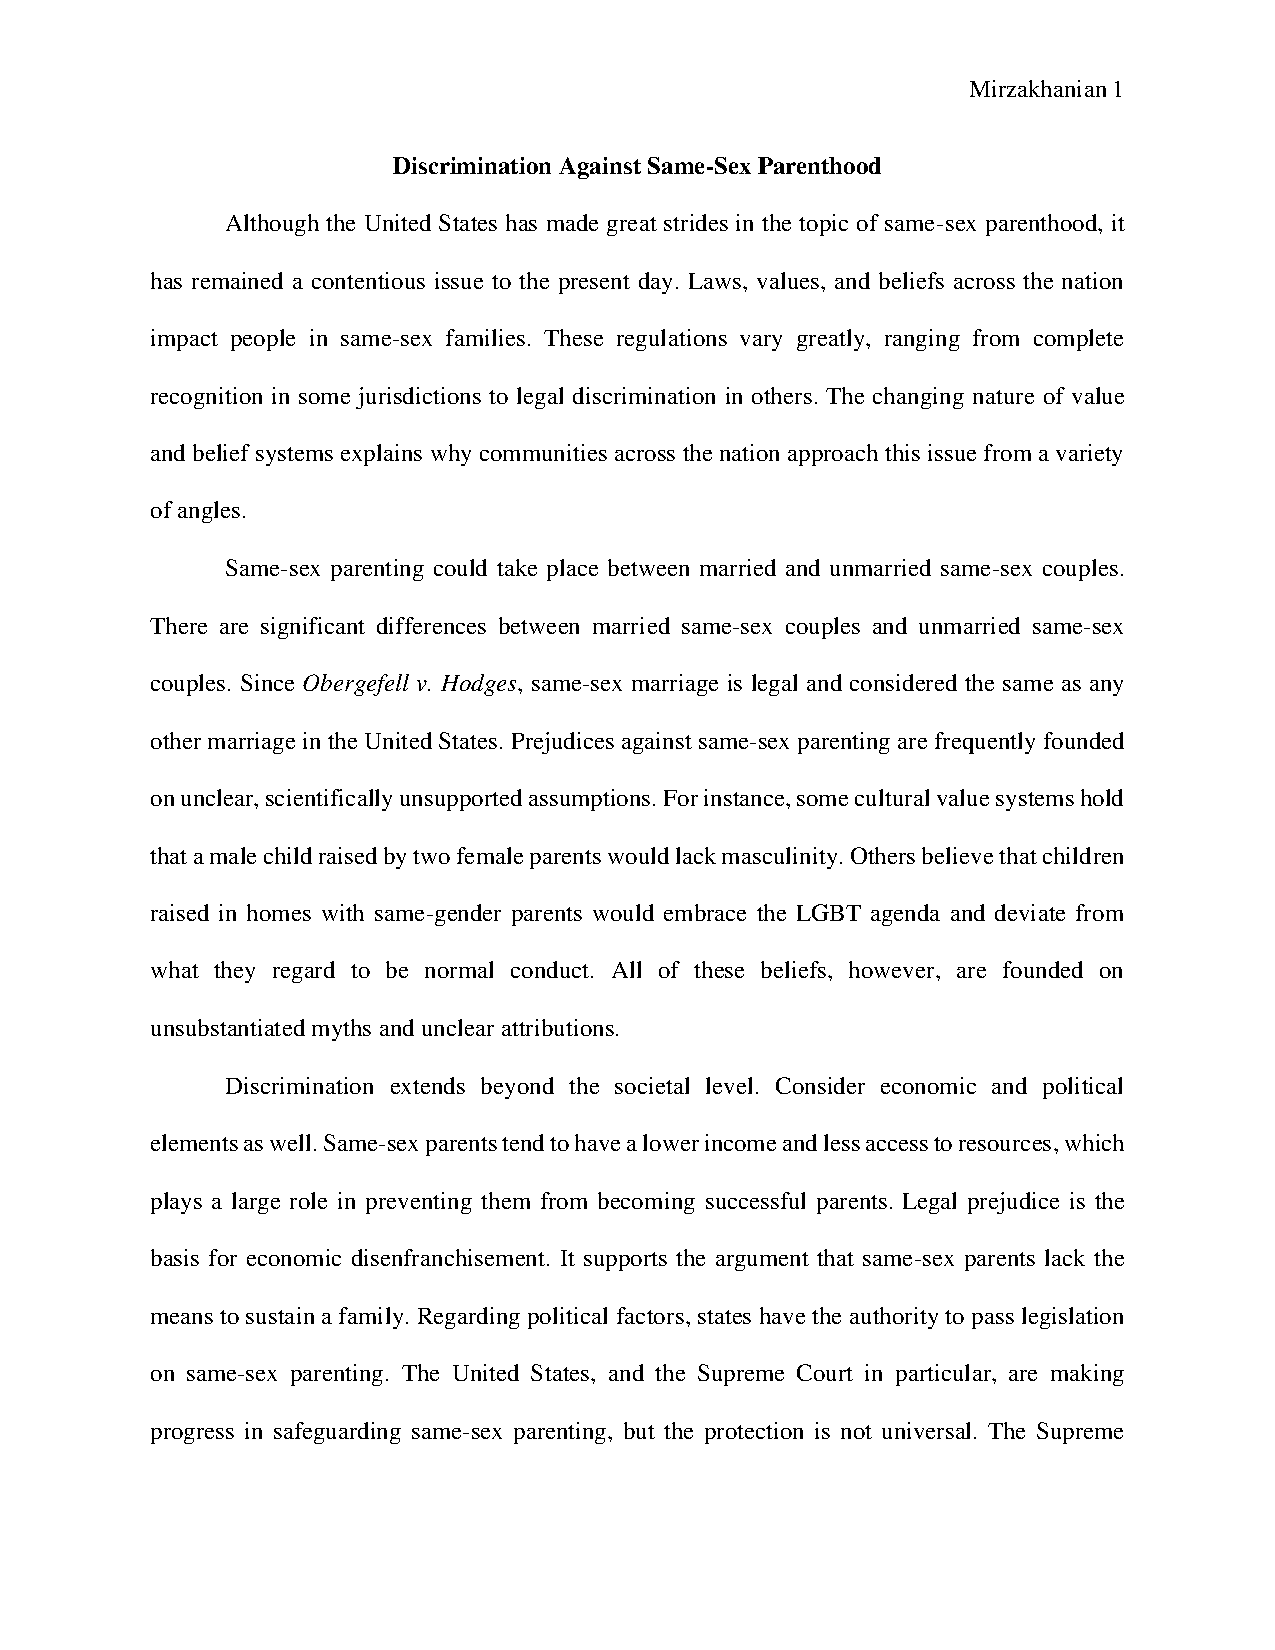
\includegraphics[width=70mm]{IROS/figs/2.pdf}}\\
  \caption{Vision localization running graph} 
  \label{figure:localization in hdmap}
\end{figure}

In recent year, many works employ a offline-built prior map to solve the vehicle localization problem \cite{2020AVP} \cite{choi2020lane} \cite{paulsmonocular}. The prior map is usually applied as a semantic or geometric representation of the scene for autonomous driving. Lidar point \cite{zhang2014loam} and vision feature point \cite{mur2017orb} are two main categories of point cloud-based prior map. Although point-cloud map can provide sufficient localization accuracy, it is environmental sensitive and difficult to provide robust localization after a long temporal period. Also, point-cloud map can not scale due to its memory requirement. Compared to point-cloud map, vector-form HD map contains precious and rich semantic geometry information. HD maps are highly structured, organized as entities with geometry and attributes. Several works explore the localization method based on HDMap \cite{choi2020lane, paulsmonocular, xiao2020monocular}. However, data association is error prone or the localization system is not complete.


To address the aforementioned problems, the goal of our method is to provide a robust and accurate vision-based localization system. %\hlr{If this is not the first work regarding vision-based localization system, this goal is too general. It would be better to give a brief but pointed description of each problem this paper aims at and the corresponding approach.}/%
We introduce a coarse to fine vision localization by combining vector-form HD map and image semantic information. In system initialization step, a coarse initialization is provided by car-equipped GPS and then refined by exhaustive pose searching. 
In tracking stage, pose is estimated by aligning image semantic perception with landmarks of same semantic meaning in HD map. Specifically, given an image or multiple images, semantic segmentation result of entities in HD map is firstly obtained by deep learning method. Based on the segmentation result, a cost map is built by utilizing distance transform like function \cite{breu1995linear}. The minimization cost can be defined as projection photometric error of landmarks on the cost map. With additional wheel odometry information, the final pose is computed by pose graph optimization in sliding-window scheme. Finally, the lost recovery module is responsible for system re-initialization when failure happens in tracking stage. The proposed system running graph is shown in Figure. \ref{figure:localization in hdmap}.

To summarize, our main contributions are:

\begin{figure*}[htb]
  \centering{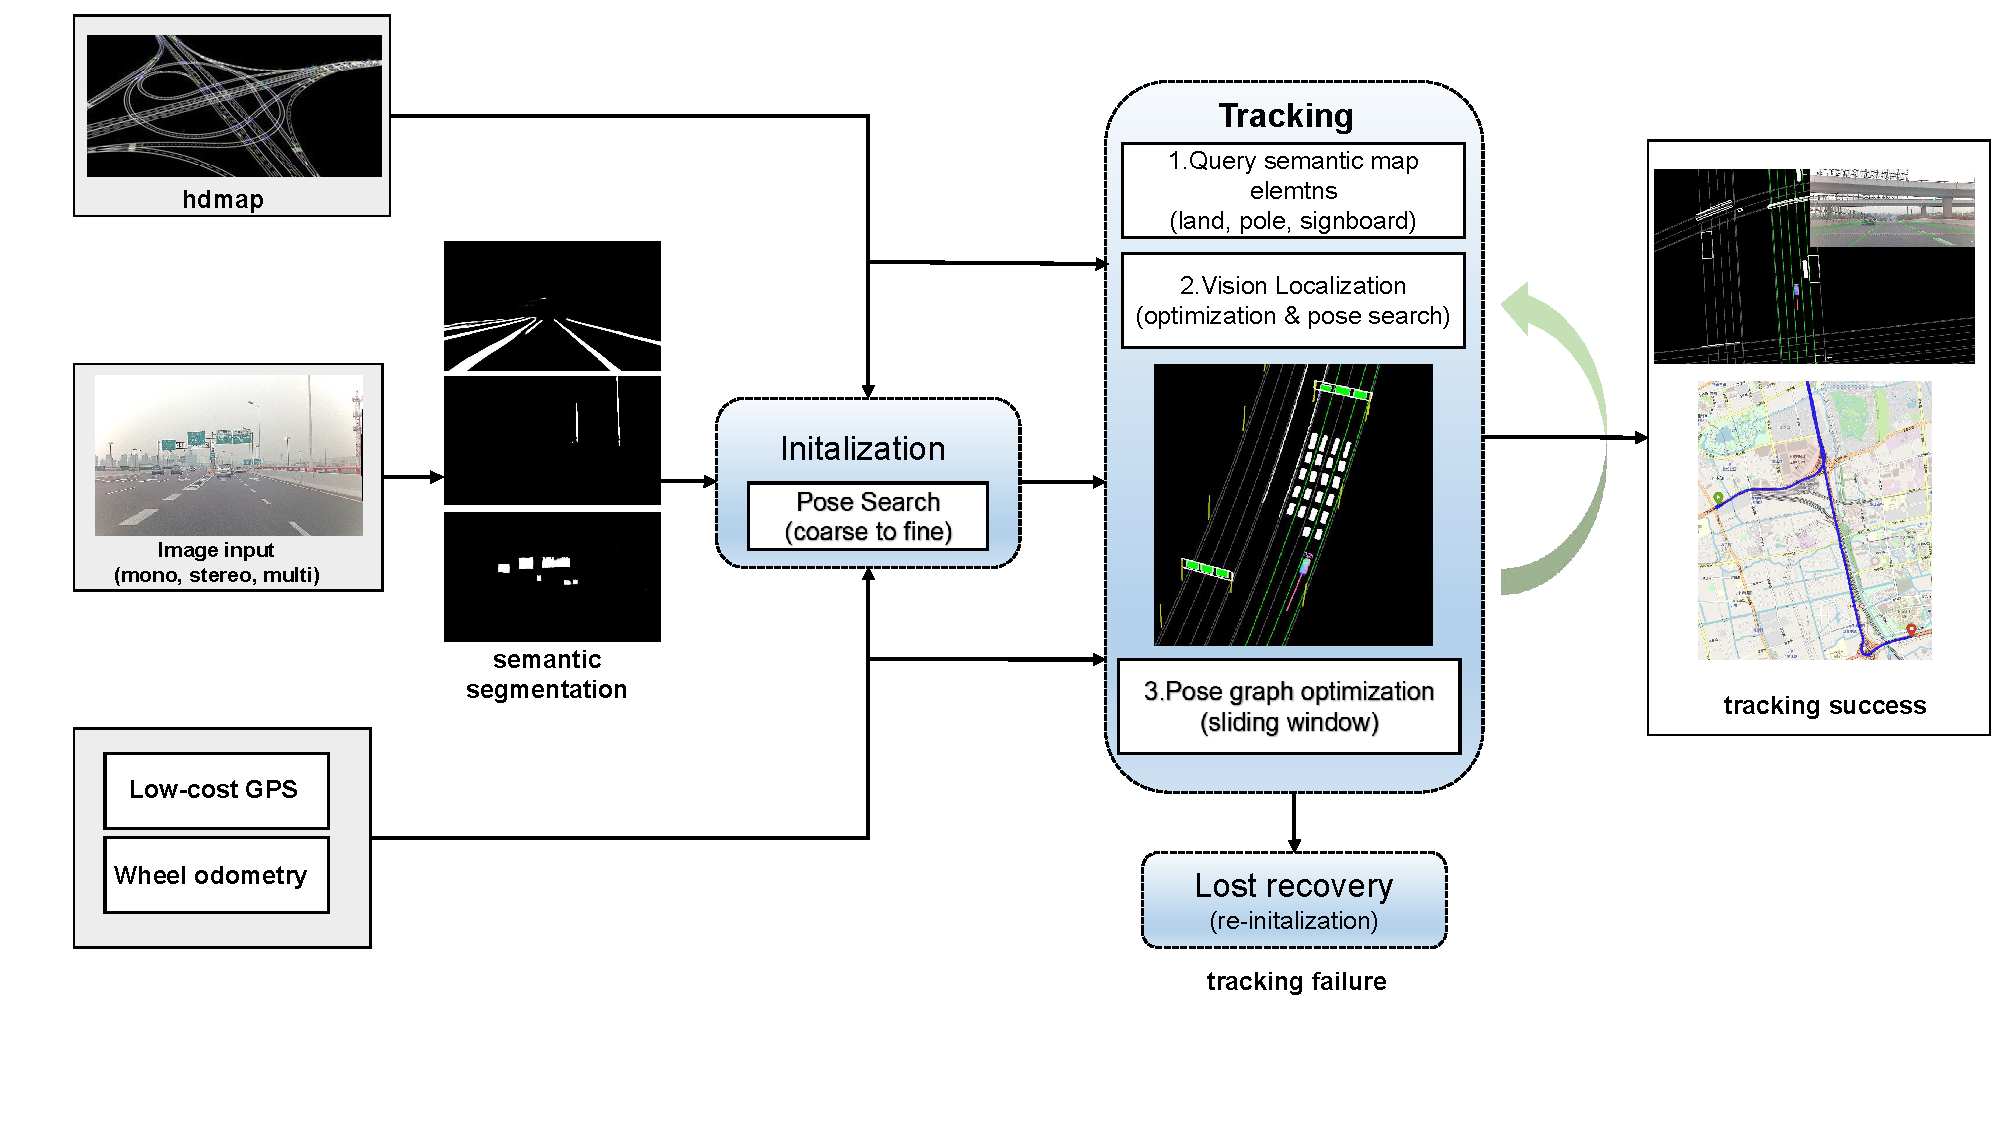
\includegraphics[width=170mm]{IROS/figs/pipeline.pdf}}\\
  \caption{Block diagram illustrating the full pipeline of the propose vision localization system. Based on the prior map, low-cost GPS and wheel odometry input, the 6-DOF pose can be estimated at centimeter-level accuracy.} \label{figure:pipeline}
\end{figure*}

\begin{itemize}

\item By leveraging semantic segmentation and HD map, we propose a complete vision localization system which includes initialization, tracking and lost recovery modules.

\item Our solution is flexible to handle both monocular camera and multi-camera system.

\item We evaluate our method on two datasets and demonstrate that our method yields promising localization results in different driving scenarios. 

% \hlr{A gentle comment: after reading the abstract and introduction, I think the current presentation is below the bar of IROS and might get rejected easily. I would like to suggest Chengcheng carefully follow some well organized and written papers to improve the manuscript significantly in the spare time after the IROS submission. This is a good opportunity to practice. If we are not lucky enough to get the paper accepted by IROS this time, when the draft is in a good shape in terms of research paper, we can still try other venues in the future.}

%\item We conduct the real-world autonomous highway pilot application based on the proposed system. The localization dataset we used will be open source for algorithm reproduction and further research.

\end{itemize}

%Semantic segmentation is used to extract features of image, including lane-marking, traffic signboard, pole-like objects and so on. Then distance transform like operation is applied in segmentation feature map to form cost image, which will be used in pose non-linear optimization. The use of cost image solve the problem of data association between map and image in an elegant way. 

%By introducing wheel odometry information constrain in the sliding window, pose graph optimization is execute to obtain smooth and robust pose output for planning and control module. Lost recovery is responsible for system re-initialization when failure happens in tracking stage. 

%With the rapid development of environmental survey technology and autonomous driving field, the vector-form hdmap is becoming a general sensor used in mass production vehicles. which expression is concise and contains rich semantic geometry information. In order to use the map effectively, we propose a novel hdmap-based vision localization method by combining vector-form high-precision map and image semantic segmentation to meet the requirements of large-scale, long-term, robust and accurate vision localization task.


\section{RELATED WORK}
%There are many research work about vision localization based on a prior environment map. Based on the method of feature association, we divide them into feature method and direct method. Based on the map format, we category them into point cloud map and vector format map.

Recently, there are many research works on vision-based localization with a prior environment map. 

\textbf{Point cloud map vs Vector-format map}
Prior map in localization can be categorized into pointcloud based map and vector-format map. The pointcloud map can be constructed by lidar or camera as sensors. Compare to point cloud map, compact vector-format HD Map is lightweight, easy to deploy and update. In order to extend the localization range, SuperPoint feature point map and semantic segmentation feature point map are both used for vehicle localization in \cite{livision}. By using lidar point cloud map, camera pose in monocular localization system, is calculated by finding correspondence between 2d lines in image and 3d lines in lidar map \cite{yu2020Monocular}. Hierarchical localization approach applies a different paradigm to finish vision localization task by introducing image retrieving into localization pipeline. For example, in \cite{sarlin2019coarse}, by matching the query image with the database images using global image feature, the correspondence between feature points of the image and the prior environment feature points map is obtained to estimate pose of query image. However, these methods are only suitable for indoor or small scale non-dynamic scenes. Many works exploits sparse semantic HD Maps in semantic localization \cite{paulsmonocular, ma2019exploiting}. Localization task is divided into two part in \cite{choi2020lane}: ego-lane identification and in-lane localization. The dash lane end point from map and image are used to localize vehicle to right position of the lane. However, only dashed lane used limits the localization application scenarios.

\textbf{Feature-based method} exploits low level geometry features or high level semantic features in the environment to build the association between image and map. Geometry feature includes point \cite{mur2017orb}, line \cite{yu2020Monocular} and plane \cite{yang2016pop}.  Camera pose can be estimated from the matching between extracted image feature and map. 
Examples of geometry features include ORB, SIFT, SURF, SuperPoint, LBD, etc. These geometry features provide distinguishing descriptions for matching task \cite{detone2018superpoint, zhang2013efficient}. However, they are not robust to environment variation, such as scenario changing from day to night or winter to summer. Therefore, they can not perform well for long-term localization. Compare to geometry features, semantics representation are alternative and widely used for localization in autonomous driving. Such representations include lane marking, curb, pole and so on \cite{schreiber2013laneloc, xiao2018monocular, xiao2020monocular, lu2017Monocular}.

%such as lane markings, curb, poles, signboard and so on \cite{schreiber2013laneloc} \cite{xiao2018monocular} \cite{xiao2020monocular} \cite{lu2017Monocular}. 

%These Geometry features such as ORB, SIFT, SURF, Superpoint, LBD and so on, has distinguishable descriptions which are key for matching \cite{detone2018superpoint} \cite{zhang2013efficient}.

%However, Geometry features are not robust to scene change. They don't have the ability for long-term localization, such as the day to night and winter to summer. Recently, semantic features are widely used in the field of autonomous driving, such as lane markings, curb, poles, signboard and so on \cite{schreiber2013laneloc} \cite{xiao2018monocular} \cite{xiao2020monocular} \cite{lu2017Monocular}. 

\textbf{Direct method} does not require explicit keypoint detectors or feature descriptors. It can naturally sample pixels from across all image regions that have intensity gradient. For example, inter-frame pose is estimated based on the image alignment of image gradient points \cite{engel2017direct}. Recently, edge features are further used to produce distance transform image for pose optimization \cite{schenk2017robust, schenk2019reslam, kuse2016robust}.

%Borrow the idea of direct method, edge features are processed based on distance transform to form gradient for optimization.
%Image edges are aligned directly by optimizing the inter-frame pose \cite{schenk2017robust} \cite{schenk2019reslam} \cite{kuse2016robust}. 

Our approach is closely related to monocular localization with HD map \cite{paulsmonocular}. 
In \cite{paulsmonocular}, image features of elements in HD map are extracted by semantic segmentation. Distance transform operation is applied on binary segmentation result of each element in HD map to generate cost image for pose optimization. Finally, cost of re-projecting map elements on cost image according to initial pose is used to optimize the camera pose step by step. However, approach in \cite{paulsmonocular} is not a complete localization system which only concludes vision tracking module. The initialization step and lost recovering module, which are essential components for localization system, are not described. Its 6-DOF optimization strategy may produce estimation error when the image information is not enough to constrain vehicle pose. The proposed system supports multi-camera sensors setup, continuous localization is performed even when some of the cameras are blocked. Furthermore, semantic feature and robust strategy are used to make the system can run in the mapped environment with challenging conditions.


\section{Method}

Given an image or multiple images $I=\{I_i\}_{i=1}^N, N \geq 1$ captured from an autonomous driving system, with a HD map $M$, the vision-based vehicle global localization is to compute 6 DOF vehicle pose $T_{wb} $. The map is defined as a set of meaningful landmark $M = \{ E_c \}_{c=1}^C$. The coordinate systems include: camera coordinate system $c$, vehicle baselink $b$ and HD map world coordinate system $w$, i.e. navigation coordinate system. Vehicle coordinate is FLU system, i.e. x axis points to forward direction, y axis points to left direction and z axis points to up direction.  Our framework consists of three major components: initialization, tracking and lost recovery. The system outputs 6DOF vehicle pose relative to the map based on the input from camera, HDMap, low-cost GPS and wheel odometry. Fig. \ref{figure:pipeline} gives the overview of our framework.

\subsection{HD Map}

High precision map in autonomous driving, is usually a simple and flexible environment structure representative of the driving scenario. We use map elements $\{ E_i \}_{i=1}^M$ lane-markings (LA), pole-like objects (PO), signboards (SB) in vehicle localization. These elements are described by successive ordered three dimensional points collection in HD map. The graph in tracking part of Fig. 2 visualizes above mentioned semantic elements. In localization system, map elements can be queried by current vehicle position and a given search radius. For queried landmarks, we sampled points with a fixed length interval as landmark representative. 

\subsection{Semantic Segmentation and Post-Processing}

In order to find correspondence between HD map elements and image, semantic segmentation is applied to extract semantic features of image. We propose a lightweight deep learning network which can provide efficient segmentation results. Typically, the backbone is Resnet-18 \cite{he2016deep} and pre-trained on Cityscape dataset \cite{cordts2016cityscapes}. The network is a multi-head structure, each head is a binary segmentation of one element (LA, PO, or SB) in HD map for localization.

The vehicle pose estimation is achieved by non-linear optimization using semantic segmentation maps. We use different post-processing methods for semantic segmentation of different elements in HD map.
Given segmentation results of lane and pole, erode and dilate operations are used for gradient image generation.
For signboard landmark, Laplace transform is applied to extract edge information, then morphology operation is used to obtain smooth gradient image. Figure. \ref{figure:dt_erode} shows the difference of cost image between distance transform and morphology operation used by proposed method. 

\begin{figure}[htb]
  \centering{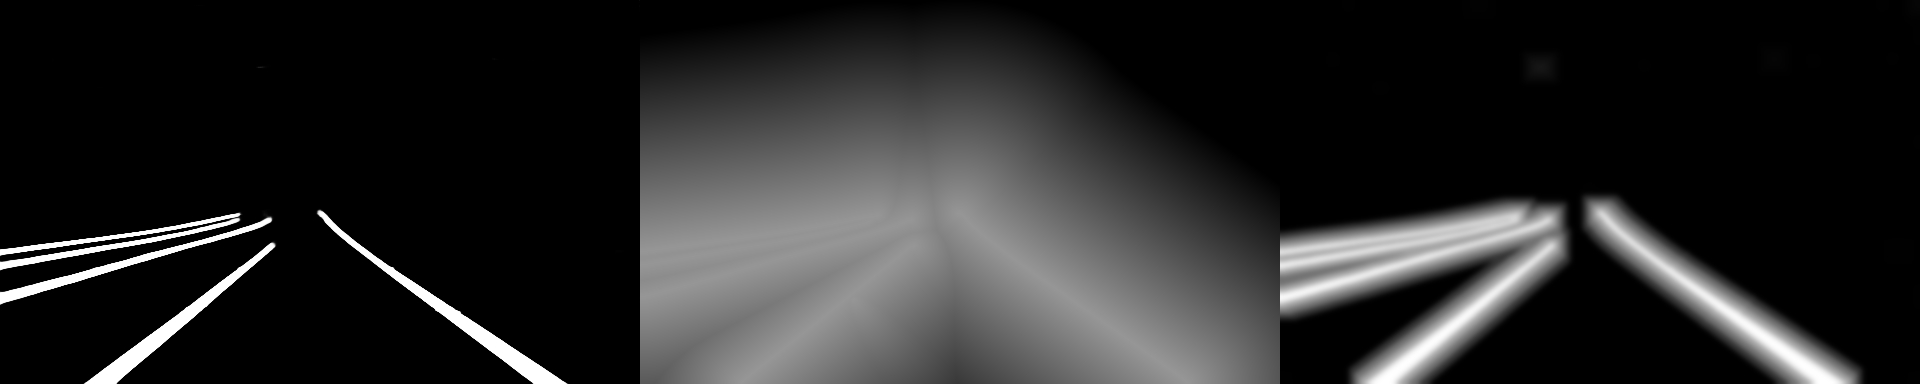
\includegraphics[width=80mm]{IROS/figs/dt_erode_1.png}}\\
  \caption{Comparison between distance transform and morphology operation. The left is raw segmentation image of lane markings, middle is the cost map based on distance transform and right is the cost map based on morphology operation.} \label{figure:dt_erode}
\end{figure}

The cost map generated by morphology is easier to make the pose optimization converge to the right result. Finally, the processed segmentation results are converted in the range of $[0, 1]$. We define the post-processed segmentation results by $I_s$.


\subsection{Initialization}
The purpose of initialization module is to obtain relative accurate pose estimation in map coordinate system for successive pose tracking step. We introduce a robust and accurate initialization method in a coarse to fine manner. Specifically, a coarse initial pose $T_{wb}$ is computed by two valid GPS records. Since vehicle can be in still status, the distance of two GPS point is set to a moderate value.
The $x$ and $y$ plane coordinate of vehicle are set to the second valid point. And $z$ coordinate is obtained based searched near map ground elements. Also, the roll angle $\theta_{x}$ and pitch angle $\theta_{y}$ of vehicle are set as zero. The yaw angle $\theta_{z}$ is set to the direction of two selected measurements. In order to get a high rate of successful initialization and more accurate initial pose result, the coarse initial pose is refined by exhaustive pose searching in a pre-defined grids.


%After above steps, a coarse pose estimation result is obtained. In order to achieve close to hundred percent initialization success rate and more accurate initial pose, the exhaustive pose searching is applied based on above coarse pose estimation.

%T is initial coarse pose and $T_{wb}$ is searched pose. $\delta state $ is the updating amount of a certain degree of the pose which depends on the pose search interval and the pose search index. 

%Initialization pose searching cost is the sum of photometric residual \cite{engel2017direct} of all semantic landmarks in map. 


The optimization cost is defined by the sum of photometric residual \cite{engel2017direct} of all semantic landmarks, which can be written as: 

%Optimal searched pose will minimize the cost, which is described by equation. \ref{eqn:photometric error}.

\begin{equation}
    cost = \sum_{i = 0}^n \|I_s(\pi((T_{wb} * T_{bc})^{-1}P_w)) - 1.0 \|_2
\label{eqn:photometric error}    
\end{equation}

In Eqn. \ref{eqn:photometric error}, $P_{w}$ is the 3d world coordinate of elements $\{E_i\}$ in the map $M$.
$T_{bc}$ is the camera extrinsic parameters relative to vehicle baselink.
$\pi$ is projection function based on the camera model. 
We use different search parameters, search step and range, for different pose freedom. For example, the search step and range for vehicle lateral position are set to 0.2m and [-10m, 10m], which covers the error tolerance of car equipped GPS. Finally, the pose combination with minimum cost will be considered as the pose of the current initialization frame. The efficient implementation is achieved by CUDA acceleration.


%The searching integral and range of the searching grid are different for each pose freedom. For example, the search interval and search range for vehicle lateral position are 0.2m and [-10m, 10m], which can cover error extent of car equipped GPS. The efficient implementation is achieved by CUDA acceleration.

\subsection{Tracking}

Given an initial pose, in tracking stage, vehicle pose is estimated based on the alignment between semantic feature and prior map. The tracking module can be divided into three steps. Firstly, vehicle pose $T_{wb}^{k+1}$ of frame $k+1$ is predicted based on pose estimation $T_{wb}^{k}$ at time $k$ and other sensor input such as vehicle wheel odemtry measurement $T_{b}^{k \rightarrow k+1}$ by:

\begin{equation}
    T_{wb}^{k+1} = T_{wb}^{k} * T_{b}^{k \rightarrow k+1}
\end{equation}

%$T_{b_{k}b_{k+1}}$ is the transform from vehicle baselink of $k$ frame to vehicle baselink of $k+1$ frame which is derived from measurements of wheel odometry. 

If the driving scenario meets the longitudinal constrain setting, a cropping local map from the global map step is performed. Otherwise, a longitudinal location correction process is applied first.


\textbf{Cropping local map from the global map} Map elements (LA, PO, and SB) are queried from the global map in a pre-defined short range using current coarse vehicle pose $T_{wb}^{k+1}$. Then the queried local map is applied for drift-free vision localization. Map element $E$ are projected back to image points $P$. In order to obtain an accurate pose optimization, points in $P$ are uniformly sampled in the image space.
%After querying the map in the short range, 
%Surrounding lane markings and road objects can be searched from current coarse vehicle pose based on map topology relationship. 
%After querying near landmarks from map, lane marking collections, pole collections and signboard collections can be obtained. This is the process which crops local map from global map. Local map is used for drift-free vision localization. 
%Due to the perspective projection of camera, points uniformly sampled in physical space are not uniform in the image space. For example, lane points in the distance are more concentrated near the vanishing point of image. For uniformly sampling in image space, every projected point will form a protect mask in image, other projected point will be discard if their projection position fall into protected mask \cite{qin2018vins}.


\textbf{Longitudinal location correction} The longitudinal localization could suffer significant drift after a long period of time, in the case that the driving scenario does not meet the longitudinal constrains. For example, it happens when the queried lanes are (1) parallel to each other, (2) straight forward, and (3) there are no signboards or poles to restrict the vehicle's longitudinal translation in the environment. GPS signal is then used to update longitudinal localization of the vehicle pose $T_{wb}^{k+1}$. Such longitudinal location correction mechanism is able to void the drift of the longitudinal localization in poor environmental conditions, especially for a long period of time.

%Therefore, the longitudinal localization suffers occur significant drift for a long time. In this situation, if GPS signal of current frame meets the preset conditions, current GPS measurement is used to update vehicle's longitudinal localization to obtain a better initial pose for successive optimization. This mechanism can ensure that the longitudinal localization will not be lost when faces with poor environmental conditions for a long time. 



%The the driving scenario does not meet the longitudinal constrains when the queried lanes are (1) parallel to each other, (2) straight forward, and (3) there are no signboards or poles to restrict the vehicle's longitudinal translation in the environment. Therefore, the longitudinal localization suffers occur significant drift for a long time. In this situation, if GPS signal of current frame meets the preset conditions, current GPS measurement is used to update vehicle's longitudinal localization to obtain a better initial pose for successive optimization. This mechanism can ensure that the longitudinal localization will not be lost when faces with poor environmental conditions for a long time. 


Secondly, the 6 DoF vehicle pose $T_{wb}^{k+1}$ is refined by image alignment with HD map elements. A cost map is built based image semantic segmentation and morphology operations. The alignment is solved by a non-linear optimization (Levenberg-Marquardt (LM) \cite{more1978levenberg}). In the case that there are missing vertical landmarks (e.g., signboards or poles) in the scene, $\theta_{y}$, $\theta_{z}$, $tx$ and $tz$ of $T_{wb}^{k+1}$ are computed by, $\theta_{z}$, $tx$ are firstly estimated and then $\theta_{y}$ and $tz$ are optimized later. $\theta_{x}$ and $tx$ are not included due to that the roll angle is usually very small when the vehicle is moving on a flat ground and longitudinal displacement of the vehicle is not observable when the vehicle and queried lanes are parallel to each other. In addition, to compromise that roll angle is missing in the optimization, vehicle rotation is then fine-tuned by a brute force search using a substantial range. Search interval of the rotation is set to 0.5 degree.


%We divide into two cases: 1) 6 dof; 
%2) 4 dof (). why: (roll, longitudinal ) not included.  
%1: (3(pitch, yaw, lateral), 2(pitch height)) why? how?

%Secondly, morphology operation is applied to segmentation image to form cost image for subsequent photometric based edge alignment optimization. Based on sampled landmark points and post-processing feature image, non-linear optimization method, such as Levenberg-Marquardt (LM) \cite{more1978levenberg}, is used to estimate the pose of vehicle. 

%If queried landmarks contain signboards or poles, 6-DOF vehicle pose is optimized. Otherwise, we split optimization process into two steps. 

%why: (roll, longitudinal ) not included. 

%Vehicle's roll and longitudinal translation are not included in optimization state. Because the roll angle is usually very small when the vehicle is moving on the flat ground. Besides, When the vehicle and queried lanes are parallel to each other, the longitudinal displacement of the vehicle is not observable.

%(1): vehicle's pitch, yaw and lateral translation are estimated. (2): on the basis of the first step, vehicle's pitch and height is further estimated. 

 
%\hlr{tune (roll, pitch, yaw, very small)}
%In addition, to compromised that roll angle is missing, vehicle rotation is then estimated by a brute force search within a substantial range.
%In addition, considering vehicle's roll angle is not estimated in above process, pose searching is used in this step again to find more accurate vehicle pose. In this step, only vehicle rotation is brute force searched in a very small range. Search range of rotation angle is set as 0.5 degree in our proposed localization system.

Lastly, in order to get a smoother pose for the planning module and to advance the robustness of the localization system, a pose graph is applied with a sliding window.
A well-tracked frame is included in the optimization window. If the window size exceeds a threshold, a frame from history will be excluded from the window  according to the vehicle state. For example, if the vehicle odometry measurement is close to zero, the second newest frame is picked, otherwise the oldest frame is used.

\begin{figure}[htb]
  \centering{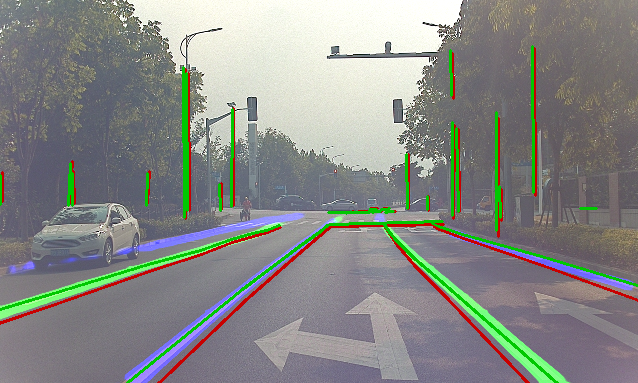
\includegraphics[width=70mm]{IROS/figs/before_after.png}}\\
  \caption{Example of Optimization. Red color stands for initial pose projection results and green color is optimization results.} 
  \label{figure:before after}
\end{figure}

In pose optimization, the factor graph has two components. The first is the prior pose factor of each frame which constrains its prior distribution of vision alignment. The other is the wheel odometry factor which establishes the connection between the adjacent frames to ensure the smooth pose output. The total residual of pose graph optimization is shown in Eqn. \ref{eqn:total cost}. The G2O \cite{grisetti2011g2o} framework is used for the optimization process.

\begin{equation}
    T = argmin \sum_{i, j \in w} \| ln(T_{i}(T_{i}^{*})^{-1})^{\vee} \|_{2} + \lambda \| ln(T_{j}^{-1}T_{i}T_{ij})^{\vee} \|_{2}
\label{eqn:total cost}    
\end{equation}

$T_{i}^{*}$ is the prior pose from semantic alignment and $T_{ij}$ can be derived from measurement of wheel odometry. A localization confidence is computed in the pose estimation to evaluate the localization status. A lost recovery module is activated when the localization fails.

\subsection{Optimization}

Details about gradient of loss function, i.e. Eqn. \ref{eqn:photometric error} are derived in following equations. Jacobian of error relative to the optimized state is usually used to accelerate the process for non-linear optimization method (e.g., Gauss-Newton or LM):

%For non-linear optimization method like Gauss-Newton and LM, jacobian of error relative to optimized state should be given for accelerate computing. The photometric based edge alignment jacobian is list in following equations.

\begin{equation}
\frac{\delta \text{error}}{\delta \epsilon} = \frac{\delta I_{s}}{\delta u} \frac{\delta u}{\delta p_c} \frac{\delta p_c}{\delta \epsilon},
\label{eqn:gradient}
\end{equation}
where \text{error} is the projection error of the cost map, ${\delta \epsilon}$ denotes the perturbation of vehicle pose, ${u}$ is the image coordinate and ${p_c}$ is the point in camera coordinate system. In order to support multi-camera observations, that optimization state is vehicle pose rather than camera pose.
The camera extrinsic parameter $T_{bc}$ is applied for the transform between vehicle and camera coordinate systems. Camera extrinsic parameters are not included in optimization state. The last term of Eqn. \ref{eqn:gradient} can be further written as:

\begin{equation}
\frac{\delta p_{c}}{ \delta\epsilon} = \frac {\delta T_{cb}(T_{wb} * Exp(\delta\epsilon))^{-1}P_{w}}{\delta \epsilon}
\label{eqn:cheap}
\end{equation}


\begin{equation}
\frac{\delta p_{c}}{\delta \epsilon} = -\left [ \begin{matrix}  I_{3} && -[p_{c}]_{\times} \end{matrix} \right] Ad(T_{cb}),
\label{eqn:cheap}
\end{equation}
where $[p_{c}]_{\times}$ is skew-symmetric matrix of $p_{c}$ and $Ad(T_{cb})$ is the adjoint of $T_{cb}$. It should be reminded that optimization state is vehicle pose rather than camera pose in order to support optimization based on multi-camera observations. Therefore camera's extrinsic parameters, i.e. $T_{bc}$ is introduced to transform point from vehicle coordinate system to camera coordinate system. For 6-DOF pose optimization, the Lie Algebra is used in transform representation.

\begin{figure}[htb]
  \centering{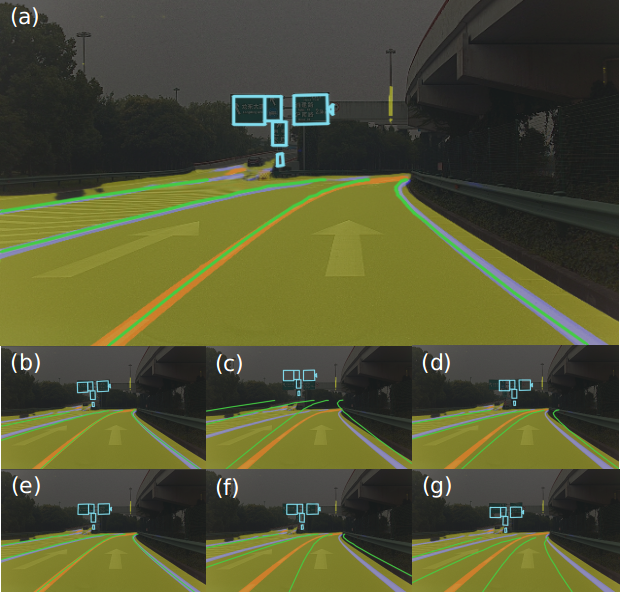
\includegraphics[width=80mm]{IROS/figs/dof_change.png}}\\
  \caption{Pose Little Change. Images are overlaid with semantic segmentation result. Yellow color stands for freespace and orange color and purple color represents lane markings. Green color is lane markings projection and cyan color is signboard projection.} \label{figure:pose vibration}
\end{figure}

3 DoF pose estimation including vehicle picth, yaw, lateral offset and 2 DoF pose estimation including pitch and height exist in the localization system. The jacobian of photometric error relative to the pose of the vehicle expressed by Euler angle needs to be derived.

\begin{equation}
    P_{c} = R_{cb}((R_{wb})^{-1}(P_{w} - t_{wb})) + t_{cb}
\end{equation}

The translation part of jacobian is list in Equation. \ref{eqn:jt}.
\begin{equation}
    \frac{\delta P_{c}}{\delta t_{wb}} = -R_{cb}(R_{wb})^{-1} = -R_{cw}
\label{eqn:jt}
\end{equation}

$\theta_z$, $\theta_y$ and $\theta_x$  are the Euler angular attitude of the vehicle body relative to the map coordinate system. In Z-Y-X rotation order, $Rbw$ is represented in Z-Y-X rotation order. The jacobian of $p_{c}$ relative to yaw can be derived. 

% \begin{equation}
%     R_{bw} = \left [\begin{matrix} c\theta_{z}c\theta_{y} && s\theta_{z}c\theta_{y} && -s\theta_{y} \\ -s\theta_{z}c\theta_{x}+c\theta_{z}s\theta_{y}s\theta_{x} && c\theta_{z}c\theta_{x}+s\theta_{z}s\theta_{y}s\theta_{x} && c\theta_{y}s\theta_{x} \\ s\theta_{z}s\theta_{x}+c\theta_{z}s\theta_{y}c\theta_{x} && -c\theta_{z}s\theta_{x}+s\theta_{z}s\theta_{y}c\theta_{x} && c\theta_{y}c\theta_{x} \end{matrix} \right]
% \end{equation}

% ``c" stands for $cos$ and ``s" stands for $sin$.

\begin{equation}
    \frac{\delta p_{c}}{\delta \theta_z} = R_{cb} \frac{\delta R_{bw}}{\delta \theta_z}(P_{w} - t_{wb})
\end{equation}

The pitch and roll part are the same principle as yaw part. Based on above derived jacobian, separate Euler angle and translation part can be optimized. All optimization process are divided into two steps. The first step is the optimization with robust kernel in order to suppress outliers. The second step is the optimization without robust kernel to obtain higher estimation accuracy by removing observations with large error in first step. Optimize result of single image is shown in Figure. \ref{figure:before after}.

\subsection{Lost Recovery}
However, the system may be lost in the following three situations: (1) vehicle is out of the operation domain of the HD map; (2) The total number of pose optimization failure exceeds a threshold; (3) The number of consecutive frames with severe occlusion exceeds a threshold (e.g, This happens in situation of traffic jam in which semantic map elements are totally invisible). The tracking confidence calculation module will determine system status based on above statistical indicators. When localization system is in lost status, lost recovery mode is activated. The pose of a lost frame is replaced by a back-up pose which is inferred from the wheel odometry, i.e. the pose before optimization. Given the next frame, in order to activate the tracking stage, the system turns into the initialization status again.

\begin{figure*}[htb]
  \centering{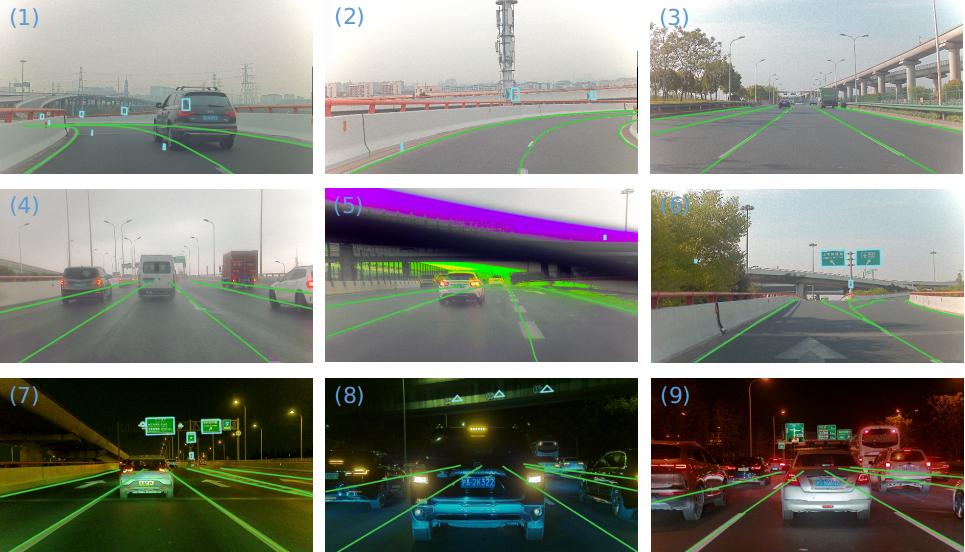
\includegraphics[width=170mm]{IROS/figs/different_scene.png}}\\
  \caption{Qualitative results on Shanghai dataset. Projection result in different scene is drawn. (1) and (2) are curve road scenes, (3) is long straight road in sunny day, (4) is in rainy day, block part in (5) is windshield wiper, (6) is diverging ramp. (7) is in low illumination scene. (8) and (9) is the scene of traffic jam.} \label{figure:different scene}
\end{figure*}

\begin{figure*}[htb]
  \centering{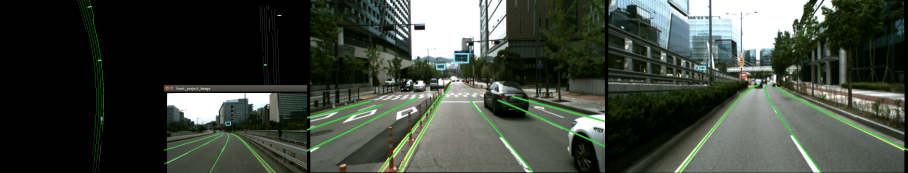
\includegraphics[width=170mm]{IROS/figs/kaist_all.png}}\\
  \caption{Qualitative results on Kaist dataset. Left is vector format landmark hdmap and projection result. Middle and right are projection results of two scenes.} \label{figure:kaist}
\end{figure*}

\section{Experiment}
The proposed algorithm is verified on two datasets. One is the elevated structured scene in Shanghai, about 30 kilometers. The map elements contained in scene include lane markings, signboard and poles which is provided by a third party map supplier. Due to the compact environment representation in vector format, the map storage size is KB level. The localization experiment is performed in different conditions, including changed weather, light intensity and routes. The other dataset is public Kaist dataset \cite{jeong2019complex}. Because Kaist dataset doesn't provide semantic map which is necessary for proposed algorithm. The stereo camera data and high-precision localization pose from Lidar and INS are used to build a semantic landmark map. Qualitative and quantitative experiments are used to evaluate the accuracy and robustness of the method.

\begin{table*}
\caption{Performance Evaluation}
\centering
\begin{tabular}{c|c|c|ccc|cc|c}
% \hline
% \multirow{2}{*}{Scenario} & \multicolumn{3}{c}{3D translation(m)} & \multicolumn{2}{c}{2D translation(m)} & rotation(deg) \\
% & max        & min        & median      & lateral         & longitudinal        & mean          \\
\hline
\multicolumn{1}{c|}{\multirow{2}{*}{Scenario}} & \multicolumn{1}{c|}{\multirow{2}{*}{frame number}} & \multicolumn{1}{c|}{\multirow{2}{*}{Init Success Rate}} & \multicolumn{3}{c|}{3D translation(m)}    & \multicolumn{2}{c|}{2D translation(m)}      & \multicolumn{1}{c}{rotation(deg)} \\ \cline{4-9} 
\multicolumn{1}{c|}{} &\multicolumn{1}{c|}{} &\multicolumn{1}{c|}{} & max  & mean  & \multicolumn{1}{c|}{median} & lateral & \multicolumn{1}{c|}{longitudinal} & \multicolumn{1}{c}{mean}          \\

\hline
sequence1   & 2470 &  $92.20\%$ &1.37       & 0.35       & 0.30         & 0.21        & 0.12       & 0.50           \\
sequence2   & 4312 & $94.24\%$ &  1.22       & 0.46       & 0.43        & 0.24        & 0.23   & 0.43          \\
sequence3   & 7490  & $85.46\%$ & 1.42       & 0.15       & 0.13        & 0.09    & 0.07     & 0.38          \\
sequence4   & 3596 & $88.79\%$ & 1.22       & 0.35       & 0.32        & 0.21       & 0.17    & 0.47          \\
sequence5   & 2289 & $73.64\%$  & 0.63       & 0.29       & 0.26        & 0.22       & 0.05    & 0.51          \\
sequence6   & 11265 & $89.40\%$ & 2.59       & 0.35       & 0.30        & 0.21      & 0.18     & 0.46          \\
sequence7   & 9297 & $90.93\%$ & 1.34       & 0.33       & 0.29        & 0.20      & 0.16     & 0.64         \\
\hline
    \end{tabular}
    \begin{tablenotes} 
		\item $\star$ This initialization success rate equals initialization success frame within 10 frames / total frames in sequence. \\
		\item $\star$ The camera of Sequence 3 is wide angle camera with 120 degree. \\
     \end{tablenotes}
    
    \label{tab:accuracy}
\end{table*}

\subsection{Qualitative}
The projection of map elements on the image should be consistent with the semantic perception if estimated vehicle pose is accurate. Figure. \ref{figure:pose vibration} show the change of map projection when the vehicle's rotation and translation deviating from original value accordingly, in which (a) is the projection result of initial pose, map elements and image perception aligns very well. The pose change of roll, pitch, yaw, x, y, z are drawn from (b) to (g) part of image. The amount of angle change is 2 degrees and translation change is 1 meter. We can see that projections of landmarks change largely when change of pitch, yaw, y and z happened. The projection results have less response to roll angle and vehicle forward direction. When estimated vehicle height is wrong, lane markings' projection will expand to image boundary or shrink to the image center. Because imaging scale is closely related to the height estimation. Based on above observation, roll angle and vehicle longitudinal position are not included in optimization state when there are no signboards or poles in searched surrounding landmarks.

Projection result of Shanghai dataset and Kaist dataset are depicted in Figure. \ref{figure:different scene} and Figure. \ref{figure:kaist}. These graphs are localization system real time running results which belong to different sequences. All the sequences in Shanghai datasets share one common HDMap which is generated earlier enough than sequences collection time. We can see that the localization algorithm is robust enough to scene change because of robust feature extraction of semantic segmentation. Proposed method is robust to landmarks occlusion for a short time period in traffic jam scene by using the backup pose induced by wheel odometry. Accurate localization result will be obtained again when landmarks can be seen from camera.

\subsection{Quantitative}
Because of the encryption of the map, the third-party map we use can't exactly match the trajectory of the high-precision trajectory of Novatel, which is a GNSS inertial navigation system. The relative pose error (RPE) is used as the metric of localization accuracy. The delta frame is 5, about 12 meter because the image capture frequency is about 10Hz, the running speed of vehicle is about 80km/h. The EVO \cite{grupp2017evo} is used as the accuracy evaluation tool. In autonomous driving field, lateral and longitudinal localization accuracy of vehicle is more considered than other metric. The longitudinal error and lateral error are calculated by our modified EVO tool.

Localization accuracy evaluations of different data sequences are listed in Table. \ref{tab:accuracy}. We can see that the accuracy is accurate to meet the demand of automated driving from Table. \ref{tab:accuracy} and Figure. \ref{figure:latlon error}. Mean rotation error is below 1 degree. Wide angle camera of 120 degree is used in Sequence 3. Localization accuracy is improved because more semantic elements are captured in lateral direction by wide angle camera. Lateral error and longitudinal error are about 20cm. Accurate projection result is helpful for semantic perception, such as traffic light and signboards detection. If the localization is successful within 10 frames by initializing from any frame in sequence, this frame will be labeled as initialization success frame. The initialization success rate can be calculated through manual labeling and observation. We can see proposed localization initialization strategy performs well, archiving about 90 percent success rate. The failure of initialization is mainly due to the poor GPS signal caused by signal blocking.


\begin{figure}[]
  \centering{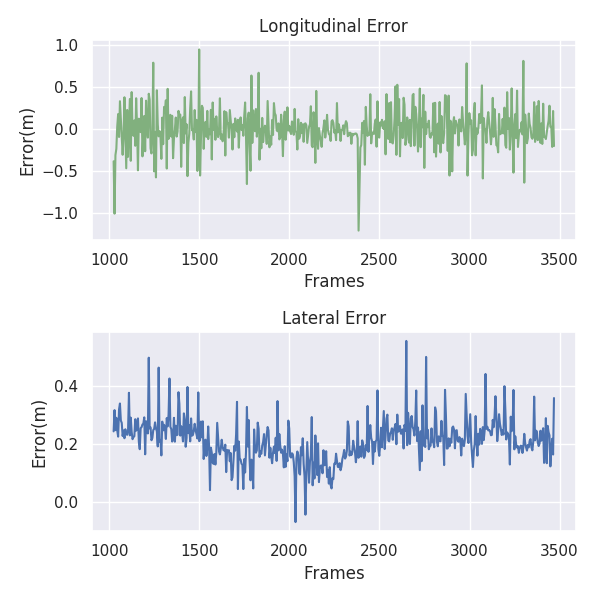
\includegraphics
  [width=60mm]{IROS/figs/lateral_lon_error.png}}\\
  \caption{Lateral and Longitudinal Error of Sequence 1} \label{figure:latlon error}
\end{figure}


\subsection{Running Time Analysis}

Table. \ref{tab:running time} show the running time statistical results of different module in the tracking part of algorithm. The time statistics don't take segmentation process into account. In the machine with i7-8700k CPU and GTX 1050 TI GPU, localization running frequency is near 100Hz. KD-Tree can be used for querying landmarks from urban scale map to improve searching efficiency. The most time-consuming step is the image post-processing, i.e. the process of gradient field construction. 

\begin{figure}[htb]
  \centering{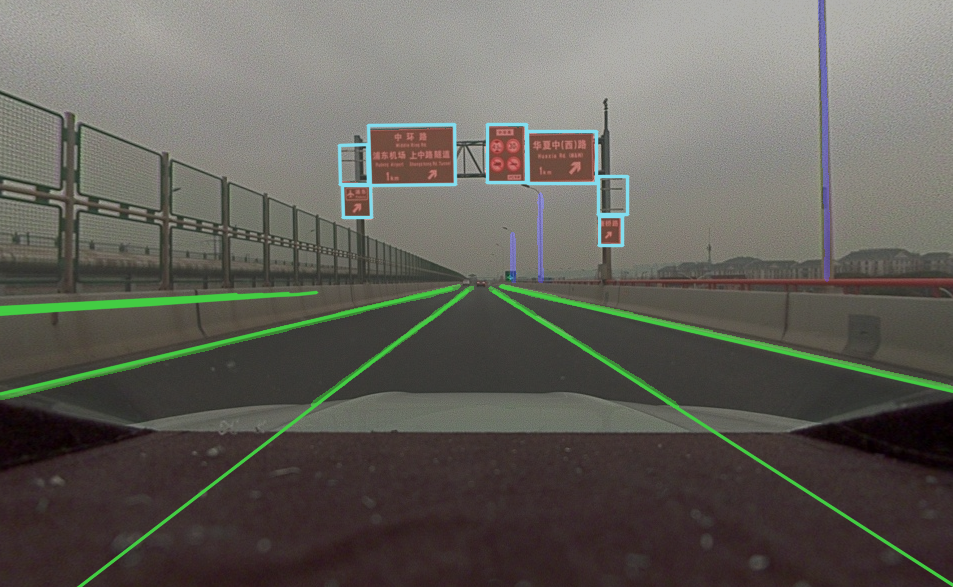
\includegraphics[width=70mm]{IROS/figs/update_map2.png}}\\
  \caption{Changed Reality Environment} \label{figure:map change}
\end{figure}

\begin{table}\small
\caption{Running time statistics.}
\centering
\begin{tabular}{c|c}
\hline
module & time(ms) \\
\hline
    image post-process &6.24 \\
    map query & 0.73 \\
    pose optimization & 1.76 \\
    pose search &0.60 \\
    total track time & 12.05 \\
\hline
    \end{tabular}
\label{tab:running time}
\end{table}

\subsection{Changed Environment}

As we all know, the update of environment mapping can't keep up with the changes of reality. However, proposed algorithm is robust to small-scale urban environment change. At the same time, the method can implicitly judge the map change region, which is conducive to the detection of map change and subsequent update. This is of great significance to the practical localization and mapping application in reality. Figure. \ref{figure:map change} shown the signboard layout change in the reality. However, the delayed map update has little influence on the vision localization results. Based on the inconsistency  between map and image semantic perception, map updating region can be recorded accordingly.


\subsection{Multi-cameras Support}

The front camera with field of view of 42.5 degree and back fisheye camera are used as our sensor setup in multi-camera localization experiment, because only fisheye camera for parking purpose is installed in our test vehicle. In order to simplify the calculation, raw fisheye image is transformed into pinhole image through the imaging model. Figure. \ref{figure:front back localization} shows localization results by using front camera and back camera and only back camera by obscuring front camera as the simulation of front camera image capture failure. It shows that even if the forward looking camera is occluded, successful localization result can still be output. Multi-cameras setup improves the robustness and accuracy of localization system.

\begin{figure}[htb]
  \centering{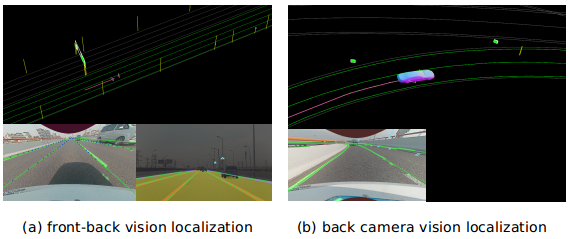
\includegraphics[width=85mm]{IROS/figs/front_back2.png}}\\
  \caption{Front camera and back camera vision localization. In (b), front camera is blocked.} \label{figure:front back localization}
\end{figure}

\section{CONCLUSIONS}

By combine vehicle wheel odometry and ordinary car-equipped consumer level GPS and HDMap, proposed method can provide accurate localization result used in autonomous driving by taking only a monocular camera as input. The propose localization initialization method can finish initialization task in almost all given coarse position, especially when signboard exists. Because the overall algorithm is designed to optimize the pose of the vehicle body by querying local landmarks from HDMap, it is not limited to the camera setup. Multi-cameras' observations in different directions can be combined to simultaneously constrain the current vehicle's pose. Semantic landmarks are stable and robust to the change of environment, including light condition, weather, traffic flow and so on. The mechanism of landmark sampling makes the algorithm not sensitive to the certain shape of landmark. Therefore, the proposed vision localization algorithm can be easily extended to urban areas by introducing more kinds of landmarks to expand the scope of application and improve the accuracy of localization.

Although the proposed method is robust, when initializing on a long, straight and symmetrical road, the cost of the lateral position in different lanes may be almost the same, resulting in setting the vehicle in wrong lane. However, the confidence calculation mechanism will make the system lost to re-initialize. When the localization elements are blocked for a long time or the current environment doesn't match the map by a large extent because of delayed map update, localization system may be failed.

In future work, we will introduce IMU into localization system, building visual inertial odometry and GNSS-IMU inertial navigation system. The pose output of VIO system and INS system will effectively fuse with the localization result of current algorithm, forming a practical low-cost mass-production localization system. 

%%%%%%%%%%%%%%%%%%%%%%%%%%%%%%%%%%%%%%%%%%%%%%%%%%%%%%%%%%%%%%%%%%%%%%%%%%%%%%%%

\addtolength{\textheight}{-12cm}   % This command serves to balance the column lengths
                                  % on the last page of the document manually. It shortens
                                  % the textheight of the last page by a suitable amount.
                                  % This command does not take effect until the next page
                                  % so it should come on the page before the last. Make
                                  % sure that you do not shorten the textheight too much.

%%%%%%%%%%%%%%%%%%%%%%%%%%%%%%%%%%%%%%%%%%%%%%%%%%%%%%%%%%%%%%%%%%%%%%%%%%%%%%%%


%\section*{ACKNOWLEDGMENT}
%We would like to thank Deshun Hu, Junhao Zhang and Yongkai %Cai for their work and great support regarding pose search %and metric evaluation as well as hdmap support from Desay %and NavInfo.

%%%%%%%%%%%%%%%%%%%%%%%%%%%%%%%%%%%%%%%%%%%%%%%%%%%%%%%%%%%%%%%%%%%%%%%%%%%%%%%%

\bibliographystyle{IEEEtran}
\bibliography{refs}

\end{document}
